\subsection{Function Shape}

\begin{figure}
	\centering
	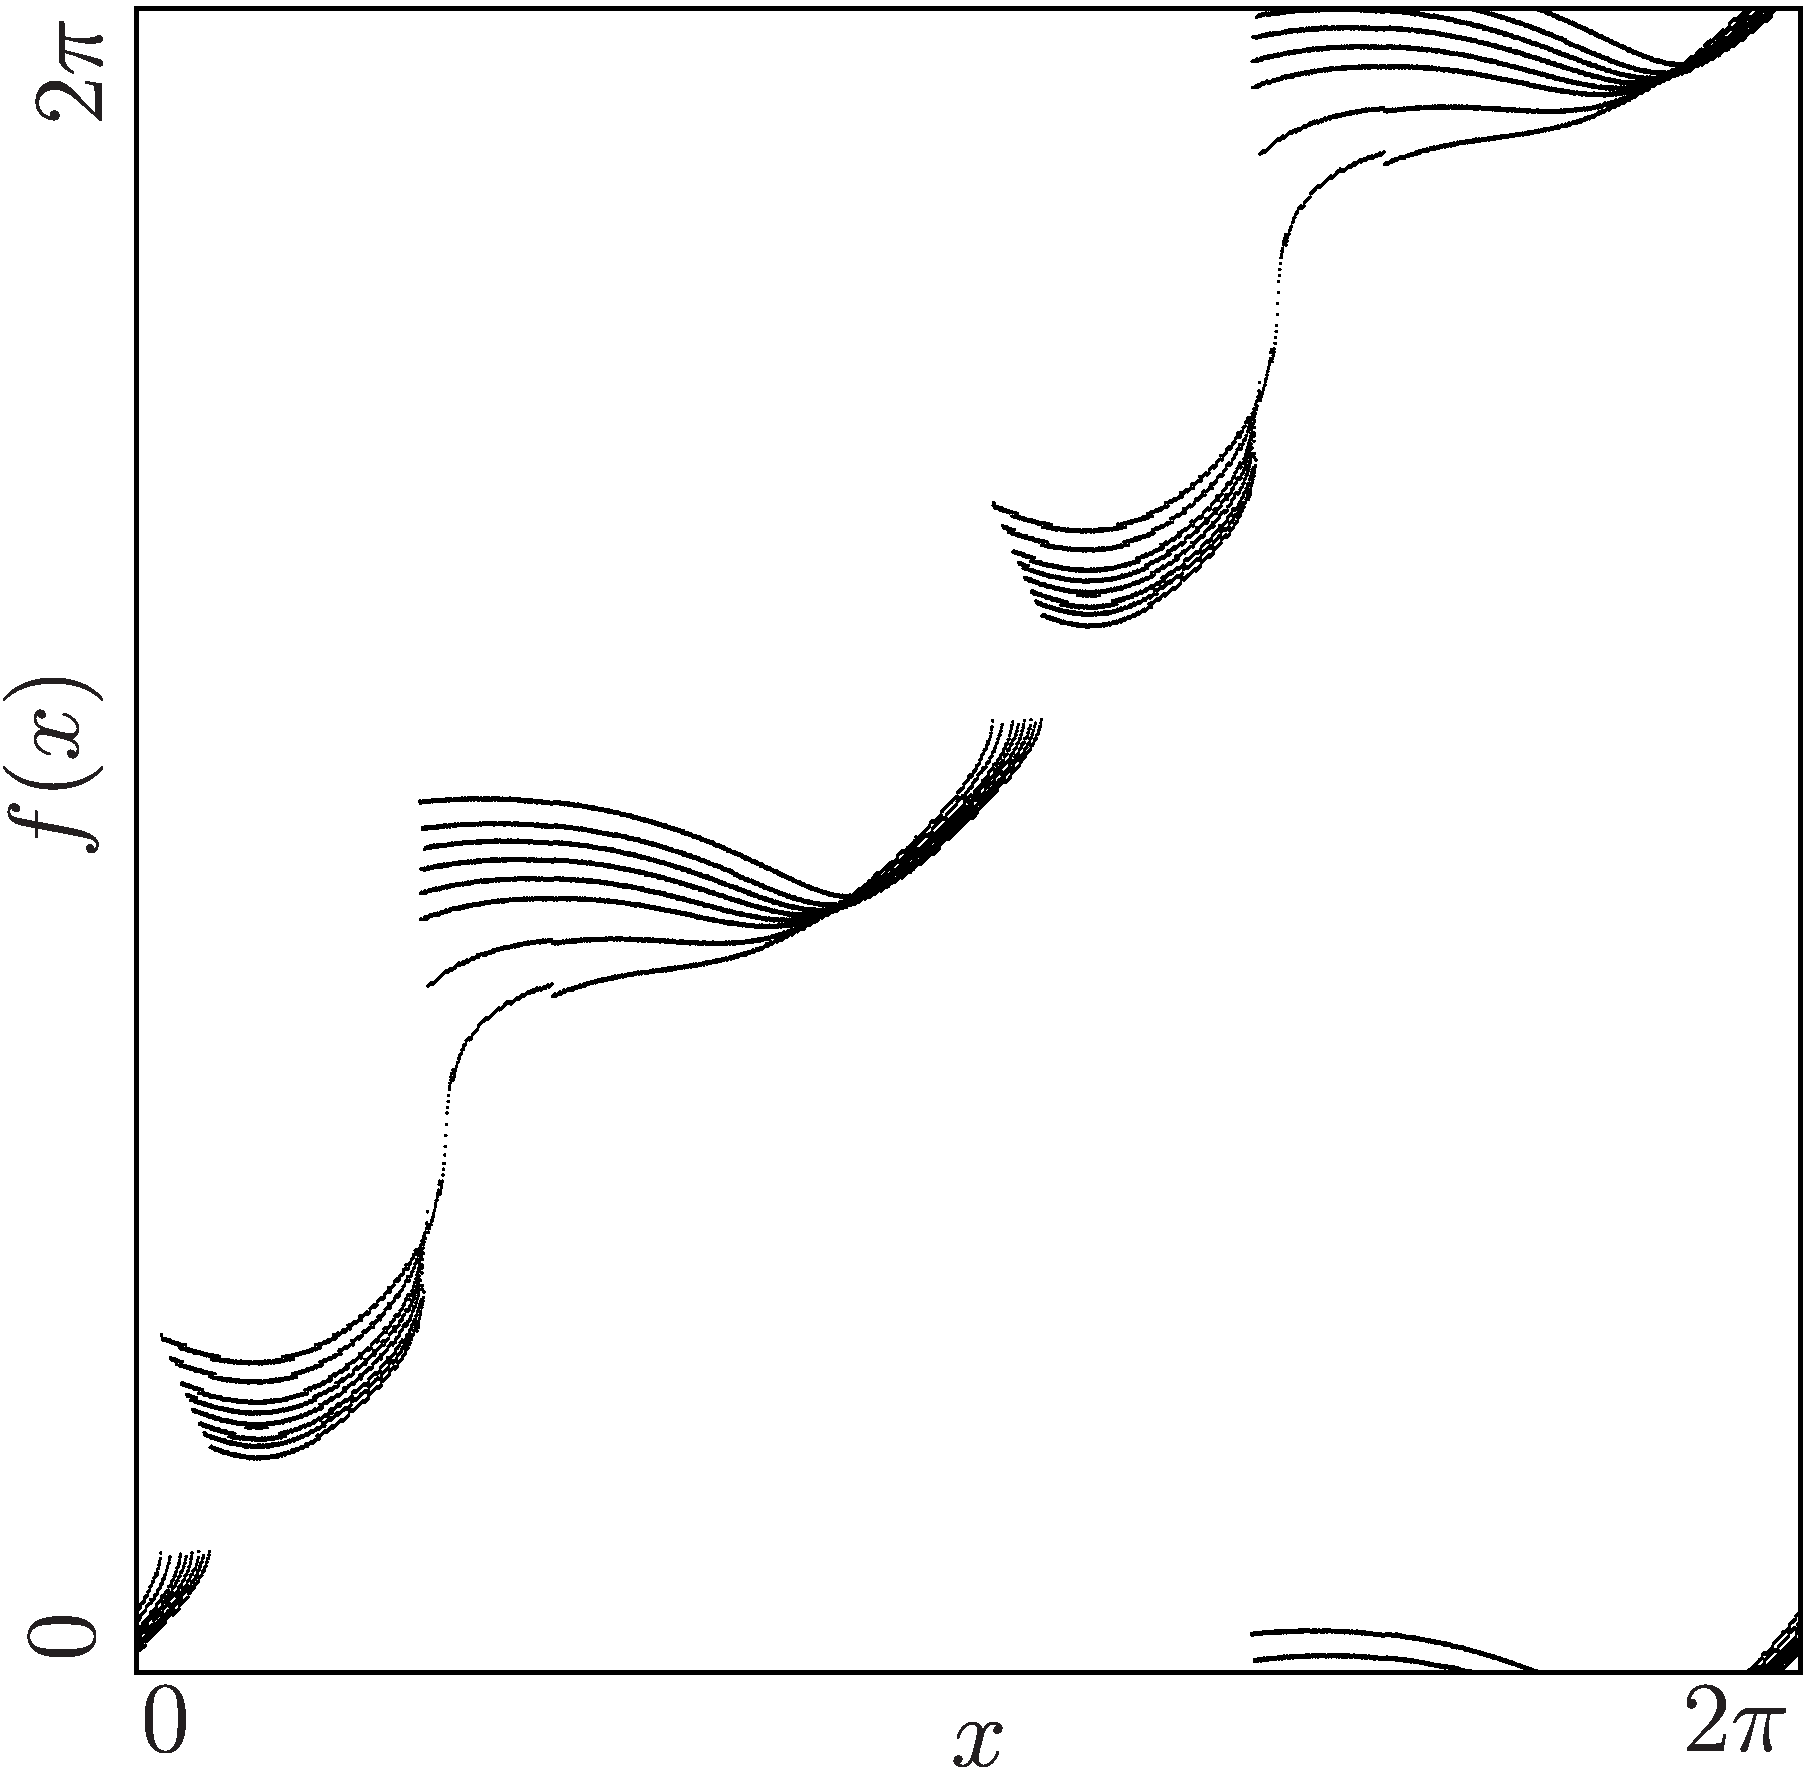
\includegraphics[width=.4 \textwidth]{99_Yunus/ParameterEffects/no/illustration.png}
	\caption[Shape of the original model function]{
		The shape of the original model function at the parameter values $E_0 = 15$ and $\chi_0 = 0.2$.
		\todo{Label branches, mayb also disc. points}
	}
	\label{fig:setup.char.shape}
\end{figure}

In this section, we examine the overall shape \hl{and number of branches} of the original model function.

\Cref{fig:setup.char.shape} shows the shape of the original model function.
We can see directly, that the \hl{model} function has 4 branches.
This is also evident from the model definition given in \Cref{sec:state.og.def}.
Also, we know from \Cref{sec:state.og.dynamics} that the model has symmetry, so the branches $F_\A$ and $F_\C$ are identical.
So are the branches $F_\B$ and $F_\D$.

There are no fixed points in the parameter regions, we are interested in.
That means, the function is always larger than the bisector $y=x$.
Also, for the most part the \hl{slope} of the function \hl{is not steep}.
\hl{
	Meaning that the absolute value of the model functions derivative is below $1$ for a majority of the state space.
	A model where the absolute value of the derivative of its model function is below $1$ for the whole state space is called contractive.
	In such a model, every fixed point and cycle is stable.
}
